\begin{figure*}[!t]
    \begin{subfigure}{\linewidth}
    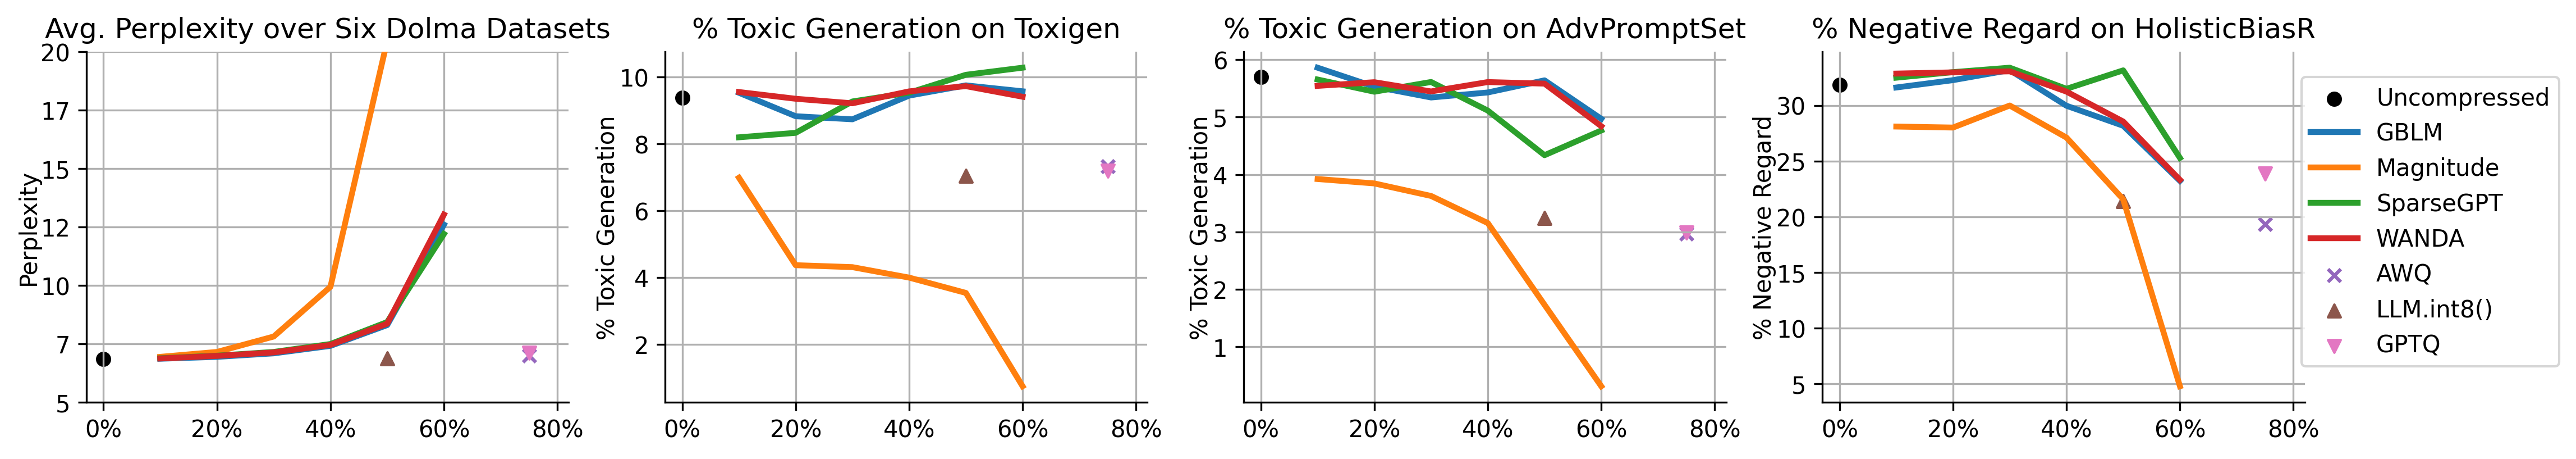
\includegraphics[width=\linewidth]{figures/A1a.png}
    \caption{Evaluation results of \llama-2-7b on language modeling, toxicity and bias datasets.}
    \label{subfig:llama2_7b_generative}
    \end{subfigure}

    \begin{subfigure}{\linewidth}
    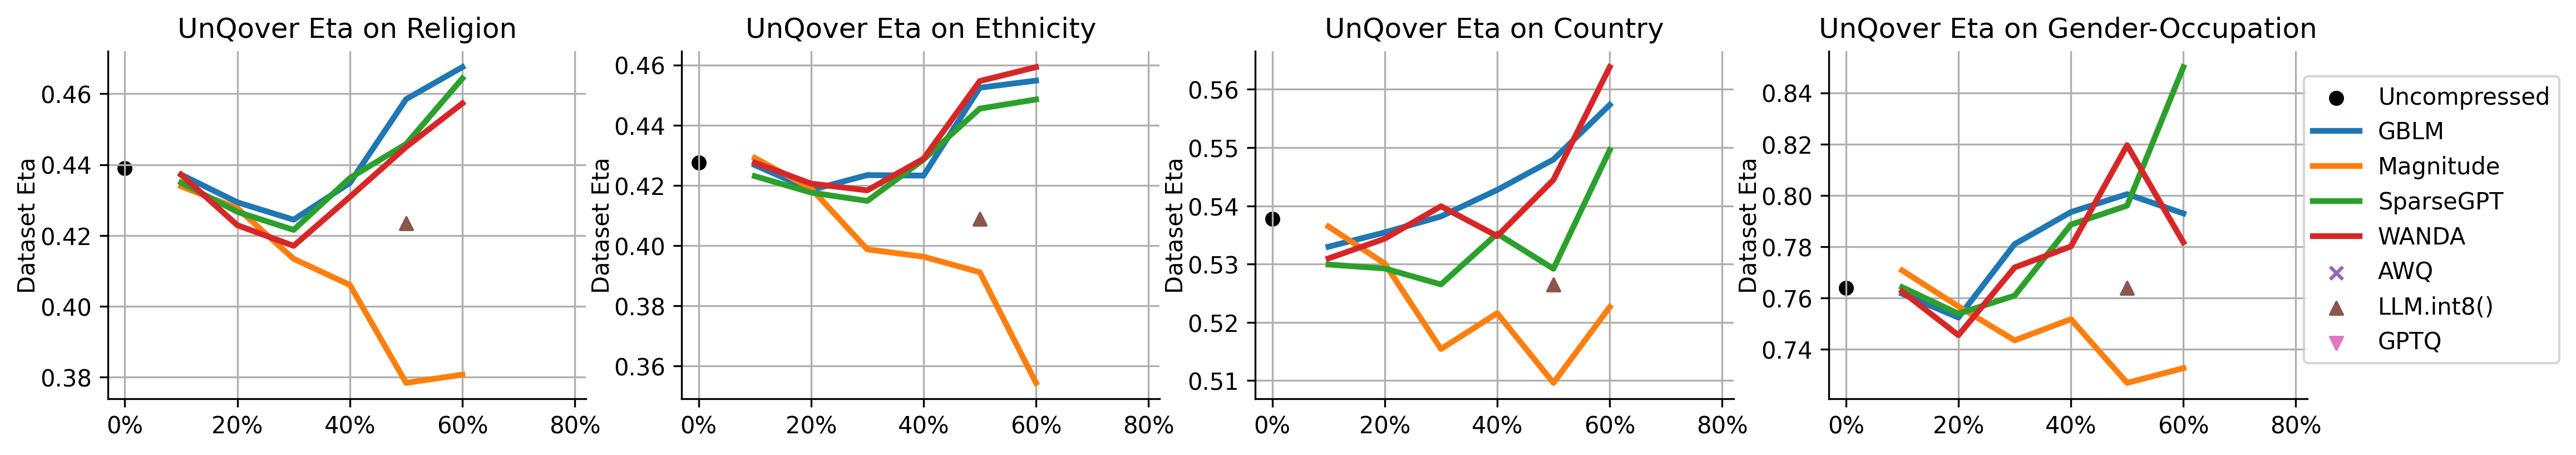
\includegraphics[width=\linewidth]{figures/A1b.png}
    \caption{Evaluation results of \llama-2-7b on \unqover~dataset.}
    \label{subfig:llama2_7b_unqover}
    \end{subfigure}

    \begin{subfigure}{\linewidth}
    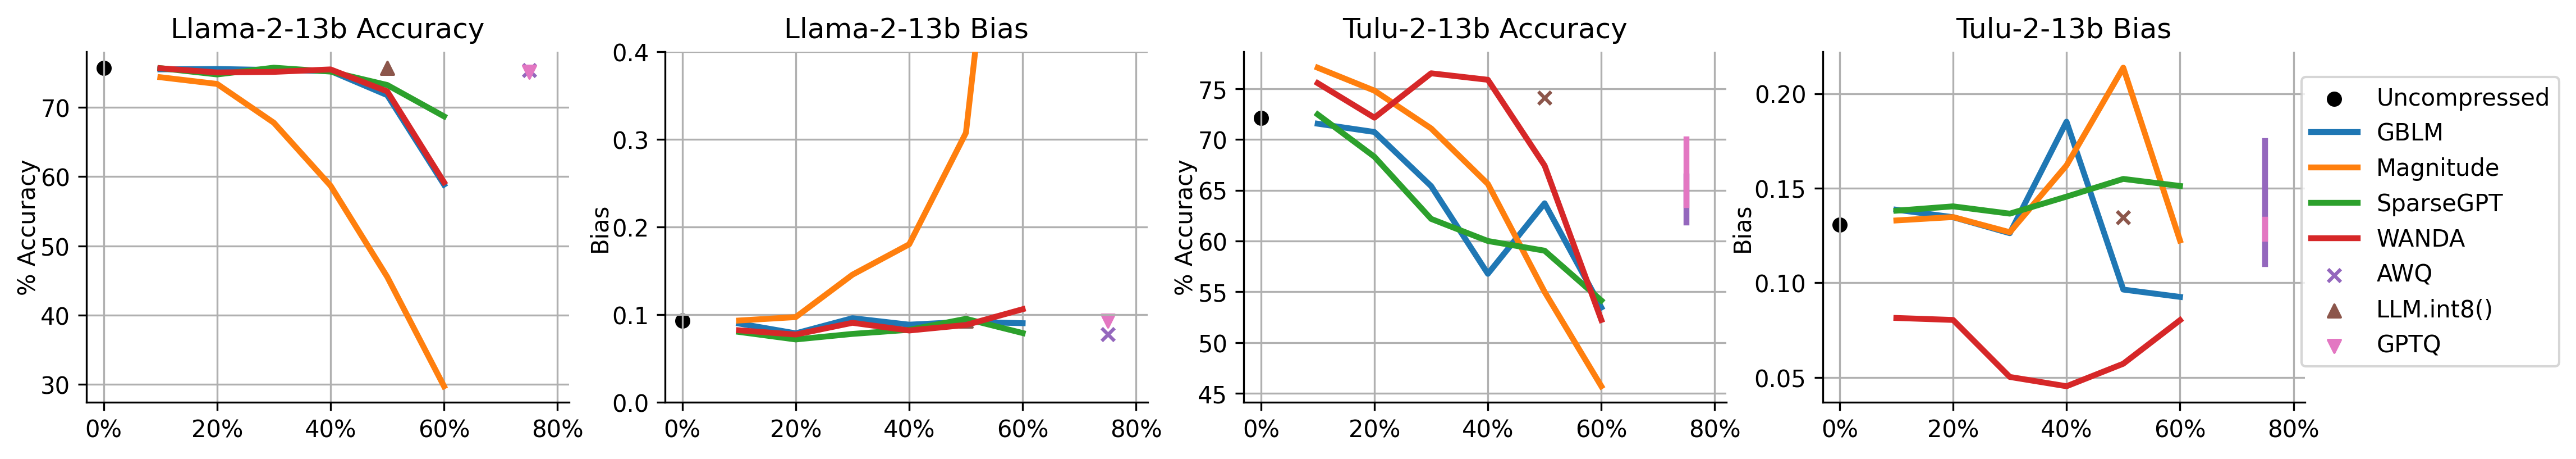
\includegraphics[width=\linewidth]{figures/A1c.png}
    \caption{Evaluation results of \llama-2-7b and \tulu-2-7b on \bbq~dataset, disambiguate questions.}
    \label{subfig:llama_tulu2_7b_bbq}
    \end{subfigure}
    \caption{\llama-2-7B's compression results on different datasets. x-axis refers to compression ratio. \bitsandbytes, \awq, \gptq~are of 50\%, 75\% and 75\% compression ratio, respectively.}
    \label{fig:llama2_7b_comprehensive}
\end{figure*}

